\chapter{Electronic Identity}

\section{Introduction}
When an information system becomes really large and complex, you need
ways to manage authentication in a unified way, because having
separate authentication systems or separate subsystem is creating
opportunities for the attackers.
In some instances, several \textbf{relaying parties}(RPs) may decide
to delegate the authentication process to a separate entity,
called \textbf{authentication server} (AS) to perform authN on their
behalf, interaction with the authN client by executing an
authentication protocol(there are several of them), and finally
providing to the RP the authN result in the form of a \textbf{ticket}
(or assertion).

Figure \ref{fig:delegated-auth} illustrates the process of delegated
authentication. In this scenario , a client seeks access to a service
provided by a relying party. An authentication server serves as the
central authority for verifying the client’s identity.  

The client begins by sending a request to the relying party. The
relying party, requiring authentication, responds with a redirect to
the authentication server, instructing the client to authenticate
first.  

The authentication server then performs an authentication protocol
with the client, which could involve methods like challenge-response,
one-time passwords, or Kerberos tickets. The outcome of this process
is communicated to the relying party, allowing it to determine whether
to grant access.  

\begin{figure}[h]
  \centering
  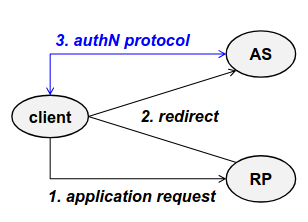
\includegraphics[width=0.5\textwidth]{img/delegated auth.png}
  \caption{Delegated authentication schema}
  \label{fig:delegated-auth}
\end{figure}

At the end of the authN process, the result is transmitted from the AS
to the RP trough various possible ways, which can vary depending on
various factors:
\begin{itemize}
  \item speed, or reaction time
  \item security and trust
  \item on services, interfaces, network filters
\end{itemize}

In the end, there's no best solution, meaning that one have to
evaluate the best solution for the specific case.
\subsection{Possible ticket transmission methods}
Let's now concentrate on the connection between the AS and the RP.
The AS can transmit the ticket to the RP in different ways, which can 
be classified in three main categories.

\paragraph{Push tickets(Figure \ref{fig:push-tickets}):} the ticket is
sent directly from the authentication server to the relying party.
This seems easy but is not that straightforward(think about network 
filters, firewalls, etc).

\paragraph{Indirect push tickets(Figure \ref{fig:inderice push
tickets}):} Since a direct communication between the authentication
server and the relying party may be impossible for various reasons, an
alternative is that the ticket is generated by the authentication
server, given to the client, and then the client will send it to the
relying party. An example of this method is Kerberos.

\paragraph{Push reference + pull tickets(Figure \ref{fig:push 
reference + pull tickets}):} the ticket reference(not the ticket
itself) is sent from the authentication server to the client, and then
from the client to the relying party. Finally, the ticket will be
pulled from the relying party. 

\begin{figure}[H]
  \centering
  \begin{subfigure}{.3\textwidth}
    \centering
    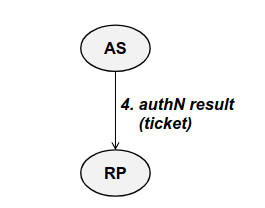
\includegraphics[width=0.9\textwidth]{img/push tickets.png}
    \caption{Push tickets}
    \label{fig:push-tickets}
  \end{subfigure}
  \begin{subfigure}{.3\textwidth}
    \centering
    \includegraphics[width=0.9\textwidth]{img/inderice push
    tickets.png}
    \caption{Indirect push tickets}
    \label{fig:inderice push tickets}
  \end{subfigure}
  \begin{subfigure}{.3\textwidth}
    \centering
    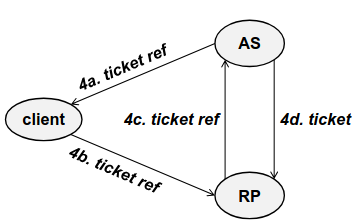
\includegraphics[width=0.9\textwidth]{img/pull ticket.png}
    \caption{Push reference + pull tickets}
    \label{fig:push reference + pull tickets}
  \end{subfigure}
  \caption{Ticket transmission methods}
\end{figure}

\subsection{Problems with tickets}
Each one of those solutions has its own problems:
\begin{itemize}
  \item binding with client, or how to bind the ticket with a 
    specific client and a specific request. If binding is not done
    correctly, replay attacks can be performed.
  \item ticket authentication, or authentication of the server from
    which is the ticket coming from
  \item ticket manipulation (at client). There are cases in which the
    ticket is passed through the client, so the client may alter that
    ticket, if not adequately protected.
  \item ticket manipulation (by MITM)
  \item ticket sniffing (in the network / at client), which exposes
    another concern: privacy!
  \item listening service at RP, which is necessary for the RP to
    listen for incoming tickets
  \item incoming firewall at RP, which can block incoming tickets 
  \item ticket replay (by same client): not only when is bound to a
    client, but also if its coming from the same client(identity
    ticket shared among multi user client)
  \item ticket reuse (at different client): is it tied to the client
    or movable to another client?
\end{itemize}

\subsection{Ticket protection}

Ticket protection is essential for securing the transmission of
tickets between the AS and the RP. 

In the case of the direct transmission between the authentication
server and the relying party, so the case of the push of the
ticket, we have different solutions.
One solution could be the creation a \textbf{digital signature} by the
authentication server that will provide authentication and integrity,
plus encryption of the data with a key possessed by the relying party.
This means full protection of the ticket.
Or if you prefer, one can create a \textbf{secure channel} where the
requirement of the secure channel which security requirements are the
authentication of the AS data integrity authentication, data
encryption and protection against replay.

In case of indirect communication, digital signature provided by the
AS and encryption for the RS is necessary and the only solution to 
protect the ticket.

More in general, protection for replay or reuse requires two things.
First of all, a timestamp, with an associated validity window(as short
as possible to still be usable). Secondly, binding the ticket with the
ID of the user that authenticated, and eventually, its network
address.

\subsection{Federated authentication}

Delegated authentication is typically performed within one single
security environment, typically within a company (like PoliTo), since
there is a very well-known set of users and RPs, and it is possible to
setup one single authentication server and all the relying parties
will delegate to that authentication server the authentication. It
does not work well when we’re in a public system like Internet, in
which we don’t know all the RP and there are several AS.

It is possible to federate the authentication among different security
domains, by using a \textbf{federated authentication system}. The
problem rely in the fact that there are various security domains, each
one managed by a different authentication server so each security
domain, internally, has got delegated authentication mechanism but the
problem is how users from one domain are able to access another
security domain. We need to create \textbf{trust relationship} so that
a relying party belonging to one domain will accept the authentication
performed by the authentication server in another domain. 

When we talk about federated authentication, unfortunately, we change
the terms. The authentication server is typically named IDP
(\textbf{Identity Provider}) while the relying party is named SP
(\textbf{Service Provider}). They are basically the same thing; the
names are related to the context.

\section{XACML}
XACML (eXtensible Access Control Markup Language) is a markup language
derived from XML designed for describing authorization policies and
managing access to protected resources. It defines policies in terms
of:

\begin{itemize}
    \item \textbf{Subject:} Entities such as users, computers, or
      services requesting access.
    \item \textbf{Resource:} Items like documents, files, or data that
      are protected and identified through URIs.
\end{itemize}

XACML also includes a language for managing access requests to these
resources. It specifies:

\begin{itemize}
    \item A structured data format to represent access request and
      response messages.
    \item Transmission over a client-server protocol of choice. After
      all, it's just a language.
\end{itemize}

XACML is an OASIS standard, with its syntax based on XML, making it
widely compatible for authorization tasks in distributed environments.

\subsection{Policy-based access control}
So, the general concept of policy-based access control it’s back to
when the IETF (Internet Engineering Task Force) wanted to have a
common way to describe admission control policies for Quality of
Services on routers. Internet infrastructure is typically multidomain,
since routers are managed by different corporations so it is needed a
common way to describe if a specific request for QoS can be satisfied
or not, after the requestor has been authenticated. So, there was an
original RFC that specified the general framework for policy-based
admission control, and then there was the COPS (Common Open Policy
Service) protocol that tried to implement that concept.

COPS was not very successful but it leaded to the foundation of what
came subsequently. After this initial attempt, there was a
generalization, an extension, to the management of information systems
(by DMTF: Distributed Management Task Force) and to the access control
in distributed environments (work performed by OASIS to apply this
concept to access control in multidomain environments).

\subsection{Components policy-based access control}
The general architecture of XACML is used for other applications, even
though XACML is not used anymore, and it's made up of four components:
\begin{itemize}
  \item  \textbf{PEP = Policy Enforcement Point}: protects a resource
    and allows access only after verification of compatibility with
    the policy
  \item  \textbf{PDP = Policy Decision Point}: receives all the data
    (policy, subject, resource, access type, context) and decides
    whether to permit or deny the access
  \item \textbf{PIP = Policy Information Point}: provides the info
    related to the access requested
  \item \textbf{PAP = Policy Access Point}: provides the policy
    applicable to the requested access
\end{itemize}

 The general architecture of a policy-based access control,
 independent of XACML, is shown if figure \ref{fig:policy access
 control}, and be implemented in several ways.

 Somewhere there is the \textit{policy repository}, where all the
 access policies are stored, which have also been created by a policy
 administrator or security manager using the PAP, which is also in
 charge of retrieving the applicable ones. Then there is a subject
 (user/router/network service) that wants to access an protected
 object. In between the subject and the object to be accessed there is
 the PEP which must decide if this kind of access is permitted or
 denied. Typically, the subject is sending a request in the form of a
 triplet
 (S,O,T):” I am this subject S, I want to access this object O, and
 the kind of access I am requesting is of this type T”. PEP does not
 know if this should be permitted or denied, so in any case it will
 block the initial request and it will talk with an appropriate
 identity: the PDP, the one that is in charge of taking a decision.
 The request MAY be (optionally) enriched with some context
 information (for example, let’s imagine that we need to know what
 time of the day is it, or where the request is physically coming
 from, for example by using geolocalization, or I could see if there
 is a direct connection or if the user is using a proxy, etc.) which
 provides more information about the kind of request and are provided
 by the PIP. Everything is
 then packed together in the form of a XACML request. Now the PDP, in
 order to take a decision, must know which policy is applicable to
 this specific case. It will query the PAP and when it will have that
 policy, it will take the decision and will send back, in XACML
 format, the response. This is mediated by the context handler, which
 has the task of translating that to the language which is understood
 by the PEP. So, finally, the response is provided to the PEP that
 will implement the response: if authorized, it will allow the 
 connection to take place.

\begin{figure}[H]
  \centering
  \includegraphics[width=0.5\textwidth]{img/policy access
  control.png}
  \caption{Policy-based access control architecture}
  \label{fig:policy access control}
\end{figure}

Notice that XACML is limited to the part in yellow in the picture, the
internal communication, because PEP is typically a kind of security
control that already exist and was considered many years ago before
XACML. The typical example of a PEP could be a firewall (network or
application firewall), or it can be any engine inside an application
that must decide if a certain action is permitted or denied, or an
Operating System in which you want to perform some operations on the
files. Those already have their own way to be configured, take
decisions, etc. That’s why normally the context handler is in place,
if not for this part (imagine we don’t need/have that), at least for
translating from a specific request format to the generic XACML. In
the end, the scope of XACML is too small.

\paragraph{Context handler}
The PEP is tightly bound to the application or service (e.g., it can
be a web server or a firewall) and it uses specific formats for
requests/responses (few PEPs are capable of using directly XACML). The
context handler converts access requests/responses from/to XACML and,
if needed, it enhances the requests with the attribute values
(obtained from PIP) often in the form of SAML assertions. When you put
some information, you want to be sure that the information is correct,
so an assertion is a strong statement: “Yes, in this moment it is
14:14:54” and it is possible to prove that, or it is possible to prove
that the user has been authenticated with his username and password.
Some strong foundation to take your decision are needed.

\subsection{XACML policy format}
A \textbf{PolicySet} serves as the primary container in an access
control system, capable of holding individual policies or other nested
PolicySets, allowing for a recursive structure. At its core, a
PolicySet must contain at least \textbf{one policy}, which defines
access control through specific components.

\textbf{Rules} within a policy establish \textbf{conditions} for
granting or denying \textbf{access}. Each rule includes an
\textbf{effect}, which determines whether access is permitted or
denied, and an \textbf{optional condition} that specifies additional
criteria to evaluate. The \textbf{target} of a policy defines its
\textbf{scope} by identifying the circumstances under which it
applies. This involves specifying the subject, the action, and the
resource.

In a Target, \textbf{Subjects} are entities described by
\textbf{attributes}, such as roles, IP addresses, or usernames. This
approach supports Role-Based Access Control (RBAC), a model that
focuses on roles within an organization rather than individual
identities, making it more flexible and scalable. \textbf{Actions}
outline the operations permitted under the policy, such as viewing,
creating, or deleting resources. \textbf{Resources} refer to the
protected entities, typically identified by URIs, that the policy
governs.


\begin{figure}[H]
  \centering
  \includegraphics[width=0.5\textwidth]{img/xacml policy
  format.png}
  \caption{XACML policy format}
\end{figure}

\subsection{XACML request format}

A request in an access control system specifies the subject, resource,
action, and environment, all derived from the request context. Each of
these elements is described through attributes, which provide detailed
information for evaluation.  

The \textbf{resource} identifies the data or object to which access is
requested. It is characterized by a set of attributes that define its
nature and context. The \textbf{action} describes the operation to be
performed on the resource, represented by its associated attributes.
The \textbf{subject} refers to the entity requesting the action,
detailed through its attributes, such as identity or role.  

Attributes serve as the foundation for defining and evaluating access.
Each attribute includes an \textbf{AttributeID}, which uniquely
identifies it, and an \textbf{AttributeValue}, which specifies the
required value for access to be granted or denied. Standard
identifiers, such as usernames, certificate Distinguished Names (DNs),
URIs, and action types, are commonly used to structure these
attributes within the system.


\begin{figure}[H]
  \centering
  \includegraphics[width=0.5\textwidth]{img/xacml request
  format.png}
  \caption{XACML request format}
\end{figure}

\subsection{XACML response format}

The response format in XACML conveys the decision made by the PDP
regarding an access request. This decision is encapsulated in the
result, which includes key elements for interpreting the outcome.  

The decision reflects the outcome of applying the policy to the
request. It can result in one of four possibilities: permit, deny,
indeterminate, or not applicable. An indeterminate decision arises
when inconsistencies or conflicts in the policy prevent a clear
resolution, where access might be both permissible and deniable
depending on the criteria. A not applicable decision indicates that no
relevant policy exists for the specific request.  

The response also includes the status, which provides additional
context about the authorization process. This status contains a status
code, a message detailing the decision, and any associated status
details. Together, these components offer a comprehensive explanation
of the PDP's decision-making process.

\begin{figure}[H]
  \centering
  \includegraphics[width=0.5\textwidth]{img/xacml response
  format.png}
  \caption{XACML response format}
\end{figure}

\section{SAML}

SAML (Security Assertion Markup Language) is a data format used for
handling authorization and authentication assertions. It is designed
to:

\begin{itemize}
  \item Represent different types of assertions.
  \item Construct requests for assertions.
  \item Represent responses containing assertions.
\end{itemize}

Again, the transport protocol is not specified: there is the object,
there is the format of the request, the format for the reply, but
transportation is left to implementation.

The core concept in SAML is the \textbf{Assertion}, which serves as
the base object to convey authentication and authorization decisions.
SAML aims to standardize and simplify interactions required to
establish permissions across a multi-domain distributed system, which
requires trust relationships.

SAML is an OASIS standard with syntax based on XML. It also provides
online tools to encode and decode various SAML formats and messages. A
helpful tool for this purpose can be found at:
\url{https://www.samltool.com/online_tools.php}.

There are various versions of SAML:
\begin{itemize}
  \item SAML 1.0
    \begin{itemize}
      \item november 2002
      \item original version
    \end{itemize}
  \item SAML 1.1
    \begin{itemize}
      \item september 2003
      \item can protect messages with XML-dsig
      \item defines profiles for web browser SSO:
        \begin{itemize}
          \item browser/artifact profile = token SAML by ref
          \item browser/POST profile = token SAML by value
        \end{itemize}
    \end{itemize}
\end{itemize}

Nowadays most of the applications use SAML2.0, which is incompatible
with the previous versions. It can still protect the messages with
XML-dsig, but can additionally use XML-enc for identifiers, attributes
and assertions (the reason is to protect the privacy of the
requestor). In addition to browser/artifact and browser/POST it has
defined new protocols, binding and profiles.


\subsection{Use cases}
Let's start to see the typical cases that have generated the various
usage of SAML.

\subsubsection{Web browser SSO use case}
A web user would like to access a protected resource of the Service
Provider (or relying party). The website does not want to implement by
itself authentication and authorization, meaning that it relies on an
Identity Provider to perform it. This is quite like the Delegated
Authentication that we discussed. This is one of the ways (the most
common) to implement it (e.g., when logging to \texttt{polito.it}, you
are always redirected to \texttt{idp.polito.it} to prove the identity,
and then, it will return an assertion about the authentication). SAML
here is used from the IDP to the SP.

\subsubsection{Authorization service use case}
This use case is very similar to the XACML one: an user is requesting
access to a resource, which access is mediated by a access control
point, the PEP, that will use SAML to check permission with the PDP.
The authorization can be returned in a SAML object (the SAML
response). So, the SAML part is in the way from PDP to PEP.

\subsubsection{Back office transaction use case}
Imagine that a professor at PoliTo want to buy something on behalf of
the university. In order to be able to do so, he must authenticate to
a authority known by both parties and be qualified to perform that
operation, receiving a SAML assertion that he can use to prove that he 
is allowed to do that. 

% 3 images 
\begin{figure}[H]
  \centering
  \begin{subfigure}{.3\textwidth}
    \centering
    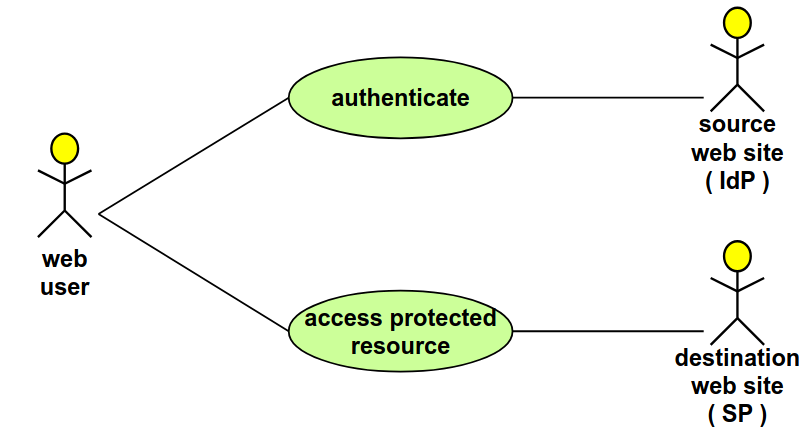
\includegraphics[width=0.9\textwidth]{img/sso use case.png}
    \caption{Web browser SSO use case}
  \end{subfigure}
  \begin{subfigure}{.3\textwidth}
    \centering
    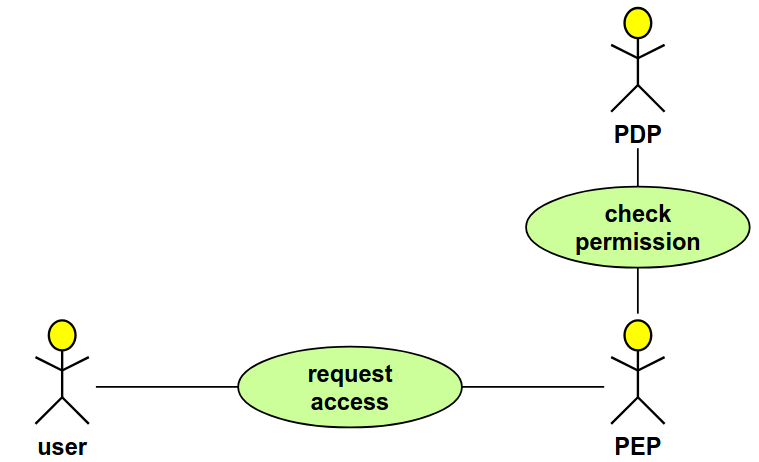
\includegraphics[width=0.9\textwidth]{img/as use case.png}
    \caption{Authorization service use case}
  \end{subfigure}
  \begin{subfigure}{.3\textwidth}
    \centering
    \includegraphics[width=0.9\textwidth]{img/back office use
    case.png}
    \caption{Back office transaction use case}
  \end{subfigure}
  \caption{SAML use cases}
\end{figure}

\subsection{SAML Assertion}

A SAML assertion is a \textbf{declaration of a fact} regarding a
subject, such as the role of a user, made by a specific issuer. There
are three primary types of assertions related to security:

\begin{itemize}
    \item \textbf{Authentication}: confirms the identity of the
      subject. This is the one returned by the Identity Provider (IDF
      – SP)
    \item \textbf{Authorization Decision}: declares whether the
      subject is allowed to access a specific resource. This is for
      the PEP-PDP communication.
    \item \textbf{Attributes}: provides additional information about
      the subject, like roles or permissions.
\end{itemize}

SAML assertions are extensible, allowing for the addition of new
assertion types as needed which can be used in a closed domain.
Additionally, assertions can be digitally signed using XML signature
to ensure authenticity and integrity. Why optionally? Because
assertions can be carried in a secure channel, like an SSL one.

\subsubsection{Information Common to All Assertions}

All SAML assertions contain the following common information:

\begin{itemize}
    \item \textbf{Issuer and Issuance Timestamp} – identifies the
      issuer and the exact time the assertion was issued.
    \item \textbf{Assertion ID} – a unique identifier for each
      assertion.
    \item \textbf{Subject} – includes the subject's name and the
      associated security domain.
    \item \textbf{Conditions} – specifies conditions under which the
      assertion is valid:
    \begin{itemize}
        \item SAML clients must reject assertions with conditions they
          do not understand (just like critical extensions in x.509).
        \item An essential condition is the \textit{assertion validity
          period}, the lifetime of this assertion.
    \end{itemize}
    \item \textbf{Other Useful Information} – may include an
      explanation or proof of the basis on which the assertion was
      constructed.
\end{itemize}

\subsubsection{Authentication Assertion}

An authentication assertion allows an issuer to declare the following
information: \textbf{the Subject S, at time T, was authenticated with
the mechanism M.}

That’s important, because in the previous course we discussed that
there are several authentication mechanisms, and they are not
equivalent: some are strong, some are weak, maybe it is possible to
combine them in a multi-factor authentication, and maybe there are
some Service Providers that will permit access only if strong
authentication has been performed, otherwise will not accept. Since
authentication is outside the control of the SP, because it is
performed by another entity (the IdP), it is needed a way to specify
back to the requestor “Yes, you are authenticated and I tell you that
I used these mechanism”, it is possible to decide if it is strong
enough or not.

\begin{boxH}
  SAML itself \textbf{does not perform the authentication process}
  (such as password requests or challenge-response interactions).
  Instead, it provides a mechanism to link to the results of an
  authentication that has already been completed by an authentication
  agent.
\end{boxH}

Now, take a look at the figure \ref{fig:saml-auth-assertion} to see
how an authentication assertion is structured. As we said, SAML is
just XML, with an opening tag \mintinline{xml}{<saml:Assertion>}. A
version major and minor fields are present, as well as the
AssertionID, which is often in the form of an IP address followed by
the date and time or the serial number. Then there is the Issuer, and
the IssueInstant fields, which will specify the date and time of the
creation (the Z at the end stands for Greenwhich Time). The second
part contains Conditions, for instance, in this case the validity time
frame. Then there is the AuthenticationStatement, which is the of the
authentication. It is made by:
\begin{itemize}
  \item AuthenticationMethod (e.g., password, reusable password, …).
  \item AuthenticationInstant: the date and time in which the user
    interacted with the IdP.
  \item Subject: NameIdentifier + SecurityDomain. Whitin the domain
    polito.it the user with username alioy has been identified.
\end{itemize}
If the issuer is trusted, then it is possible to accept this as a
proof that the user was authenticated. Of course, there are problems
of trust: if that has been manipulated, how it is transmitted, so the
transmission of this SAML token goes back to the discussion of the
previous pages about how to transfer the result of the delegated
authentication.

\begin{figure}[H]
  \centering
  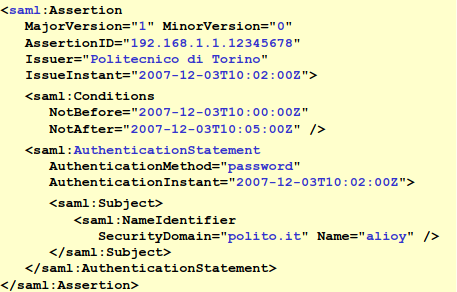
\includegraphics[width=0.6\textwidth]{img/saml auth assertion.png}
  \caption{SAML authentication assertion}
  \label{fig:saml-auth-assertion}
\end{figure}

\subsubsection{Attribute Assertion}

An attribute assertion allows an issuer to declare the following
information: \textbf{the subject S is associated with one or more
  attributes (attributes A, B, C, …) that currently (in this moment)
  have the values “a”, “b”, “c”, … }

\noindent These attributes are typically obtained through an LDAP
query.

\noindent \textbf{Example:} The subject "alioy" within the domain
"polito.it" is associated with the attribute "Department," holding the
value "DAUIN."

Take a look at the figure \ref{fig:saml-attribute-assertion} to see
how an attribute assertion is structured. 
The Initial tag and Conditions are the same as in the previous
example. Then, it is specified that the example is an
AttributeStatement, in which there will be a different content. The
NameIdentifier is the same as before (security domain + name). Then in
the Attribute part there will be the AttributeName “Dipartimento”,
again in the specified namespace (because each namespace may have
different attributes) and the value will be DAUIN. So, if the system
manager is performing Role Based Access Control, it is possible to say
something like “Everybody which belongs to a certain department can
access, for example, the portion of the information system related to
that department”. This is the way in which is possible to know that a
user belongs to that department.

\begin{figure}[H]
  \centering
  \includegraphics[width=0.6\textwidth]{img/saml attribute
  assertion.png}
  \caption{SAML attribute assertion}
  \label{fig:saml-attribute-assertion}
\end{figure}

\subsubsection{Authorization decision assertion}
Finally, to implement the PIP-PDP model, there is the authorization
decision. An issuer declares that \textbf{it has taken a decision
  regarding an access request made by a subject S for an access of
  type T to the resource R based on the evidence E}.

The S, T, R elements are the access request, while the E is important
for taking care of why the permission has been given/denied. For
example, it could as a minimum say “this is based on
polito.it.policy.2.5”, because maybe the policy will change in the
future and by specifying it there will be an evidence that in that
version there was the allowed access to anybody of the DAUIN
department for the resource. The subject can be a person, a program
and a resource can be everything (e.g. a web page, a file, a web
service etc.).

Take a look at the figure \ref{fig:saml-auth-decision-assertion} to
see how an authorization decision assertion is structured. 
The initial tags are the same as before, but in this case there will
be the AuthorizationStatement, in which there will be the decision
field to specify if it is permitted to access the specified resource
(\texttt{http://did.polito.it/m2170.php}) from the person specified in
the Subject (the one corresponding to name alioy in the domain
polito.it). In this case the evidence part is not specified. It means
that the decision has been taken and it is not conveying in the
assertion why the decision has been taken in that way.

\begin{figure}[H]
  \centering
  \includegraphics[width=0.6\textwidth]{img/saml authorization
  decision assertion.png}
  \caption{SAML authorization decision assertion}
  \label{fig:saml-auth-decision-assertion}
\end{figure}

\subsection{SAML producer-consumer model}
These different kinds of assertions are related. By looking at the
last example (authorization decision assertion) it is possible to
notice that the subject is specified, but has the subject
authenticated? If authentication is needed, it means another assertion
is needed.

The assertions can be used individually, but they are quite often used
together, which leads to the general schema presented in figure
\ref{fig:saml produce-consumer model}, in which there are several
entities that at the same time are producing an assertion but also
consuming (receiving) an assertion. 

The schema contains three types of available assertion in the SAML
part. The authentication assertion is from an authentication
authority, the attribute assertion is from an attribute authority but
notice that before deciding which is the attribute it is needed to
know who is the requestor, and the Policy Decision Point is creating
an authorization decision, but this could be based on the identity of
who is requesting and maybe on the attributes (maybe “Lioy” is not
enough, which Lioy? From which department?) and the authorization
decision is used by the \textbf{Policy Enforcement Point}. Each of them (the
authorities) has got a specific policy, for example the
authentication method, and then there is some system entity (which can
be a user, or a program) that performs an application request, the PEP
will block (control) the access to the SP and the system entity in
order to get access must perform authentication (maybe trough a
Credentials Collector or an Authentication Protocol) and then the path
showed in the picture will start.
\begin{figure}[H]
  \centering
  \includegraphics[width=0.6\textwidth]{img/saml produce-consumer
  model.png}
  \caption{SAML producer-consumer model}
  \label{fig:saml produce-consumer model}
\end{figure}

\subsection{SAML: protocol for the assertion}
SAML is not only describing the format of the assertion itself but is
also specifying how the request and the response are created (but not
how they are transported).

The assertion will be contained in a SAML container and will be put in
a Response. The request must be created for that specific type of
assertion, and that is created between the relying party and the
asserting party. It is used “relying party” because it relies upon the
asserting party being a trusted source of information, so it relies on
the assertion created by the asserting party to implement its own
functionality.

\begin{figure}[H]
  \centering
  \includegraphics[width=0.4\textwidth]{img/saml assertion
  protocol.png}
  \caption{SAML assertion protocol}
\end{figure}

\subsubsection{Request of authentication assertion}
The request of authentication assertion is conceptually something of
the kind “please, give me authentication information, regarding this
subject, if you have any”. It is assumed that requestor and the
responder have a trust relation, because they speak about the same
subject and the response is a sort of recommendation letter: “yes, it
is possible to trust this user because I have authenticated it”.

An example of request of authentication assertion is shown in figure 
\ref{fig:saml-auth-assertion-request}.
In the picture the example shows now \mintinline{xml}{<samlp>} where p
stands for protocol. The content will now be an AuthenticationQuery
which asks for information about the specified user. It is something
like: “please tell me if you have authenticated this guy that pretends
to be alioy in the domain polito.it”.

\begin{figure}[H]
  \centering
  \includegraphics[width=0.5\textwidth]{img/saml auth assertion
  request.png}
  \caption{An example of request of authentication assertion}
  \label{fig:saml-auth-assertion-request}
\end{figure}

\subsection{Trust relationship}
The assertion is part of a triangle between to the parties: user, service
provider and the identity provider. 

The one who accepts the assertion must trust the entity that generates
an assertion. The trust relation is established by pushing or direct
pull on a secure channel (e.g., TLS), which may be established with
mutual authentication or at least the asserting party must
authenticate itself. If a TLS channel is not used or if it is wanted
to maintain a proof of the assertion, it is possible to use
XMLsignature over the SAML object using a shared (MAC) or public key
(real digital signature). The last case is a long-term solution while
the TLS channel gives a temporary trust.

\subsection{Binding SAML}
SAML defines \textbf{"what"} to transport, while the binding defines
\textbf{"how"} to transport it, i.e., a network protocol for SAML
requests and responses.

\begin{itemize}
    \item SAML/SOAP(Service oriented architecture protocol)-over-HTTP
      is the original binding in version 1.0.
    \item SAML 2.0 defines other bindings:
    \begin{itemize}
        \item SAML SOAP binding (based on SOAP 1.1)
        \item Reverse SOAP (PAOS) binding
        \item HTTP Redirect (GET) binding
        \item HTTP POST binding
        \item HTTP Artifact binding
        \item SAML URI binding
    \end{itemize}
\end{itemize}

\subsection{SAML Profiles}
A SAML profile is a concrete manifestation of a defined use case using
a particular combination of assertions, protocols, and bindings. 

In practice a profile is like a software pattern (design pattern)
which is a standard way to implement something relative to important
information for a specific use case:
\begin{itemize}
  \item Web browser profile is needed to implement Single Sign On
    (SSO) web
  \item SOAP profile is used for assertion about the SOAP payload – in
    case it is used
\end{itemize}

\subsection{SAML and SOAP}
Typically, we have SAML that contains a SOAP message with the SOAP
header, SOAP body, and the request and response are carried inside
this protocol. So it actually is layered in three protocols: SAML
inside SOAP inside HTTP.

Figure \ref{fig:soap-profile} shows how the SOAP profile is 
structured. 

% 2 subfigure 
\begin{figure}[H]
  \centering
  \begin{subfigure}{.4\textwidth}
    \centering
    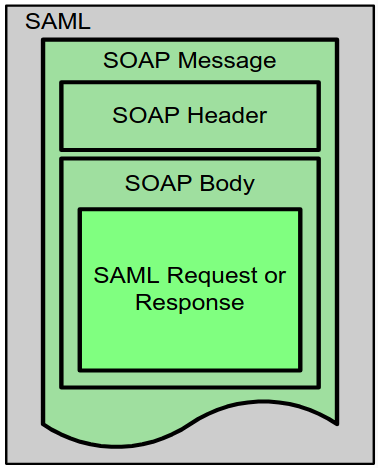
\includegraphics[width=0.9\textwidth]{img/soap over http.png}
    \caption{SAML over SOAP over HTTP}
  \end{subfigure}
  \begin{subfigure}{.4\textwidth}
    \centering
    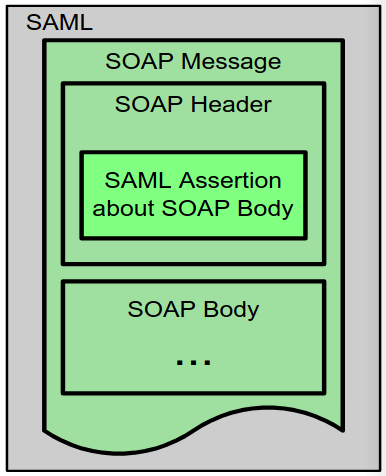
\includegraphics[width=0.9\textwidth]{img/soap assertion.png}
    \caption{SOAP profile}
    \label{fig:soap-profile}
  \end{subfigure}
  \caption{SAML and SOAP}
\end{figure}


\subsection{Web Browser Profiles}

Web browser profiles, which are surely more relevant nowadays, operate
under the following assumptions:
\begin{itemize}
    \item A standard commercial browser and HTTP(S) are used.
    \item The user has authenticated with a local source site.
    \item The assertion’s subject implicitly refers to the user.
\end{itemize}

When a user tries to access a target site:
\begin{itemize}
    \item A small authentication assertion reference is included with
      the request, allowing the real assertion to be dereferenced.
    \item Alternatively, the real assertion is directly POSTed.
\end{itemize}

The choice between these methods is determined by the agreement
between the Service Provider (SP) and Identity Provider (IdP).

\subsection{SSO use case}
\subsubsection{SSO push use case}
The procedure is shown in figure \ref{fig:sso-push-use-case}. The the
client (browser) is trying to connect  to a specific page of a web
server (which is the SP). The resource is protected, so a redirect is
received (HTTP codes that start with 300). The SP has a specific
agreement with an Identity Provider like the case of PoliTo and is
redirecting there with an authentication request, which is hidden
inside the redirect. It means that when the client goes to the
Identity Provider it is automatically transmitting this authentication
request (number 3 in the picture) which is not created by the client,
but it is a consequence of the redirect.

The Identity Provider is implementing some kind of authentication
protocol (username and password, OTP, challenge response etc.) and
will finally create the answer and it must return the answer to the
Service Provider.


Assuming that it is successful, then will create for you a form that,
when you hit the Submit button, will send you to the service provider.
Inside this form, as hidden data, there will be the authentication
result. When the client wants to go back to the Service Provider, it
will automatically (involuntarily) transmit the authentication
response (number 6, again it is not created by the client). This is
the push use case (with reference to the delegated authentication),
because the IdP is pushing the token (which is the SAML assertion) to
the SP. Finally, the SP (if authN was successful) will provide the
requested service to the client.

It is also named front-channel exchange because it directly uses the
channel towards the SP.

\begin{figure}[H]
  \centering
  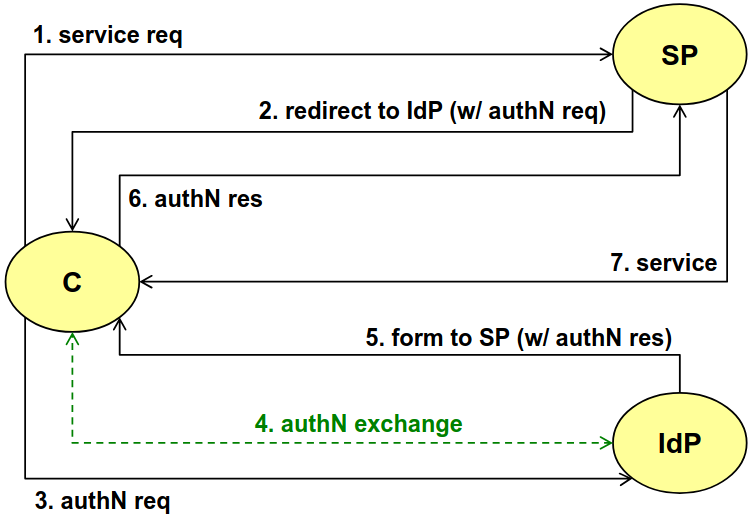
\includegraphics[width=0.5\textwidth]{img/sso push use case.png}
  \caption{SSO push use case}
  \label{fig:sso-push-use-case}
\end{figure}

\subsubsection{SSO pull use case}
In the SSO push use case all data are transmitted using the same port
(there will not be an alternate port).

In this case, the first stages are the same as before: service
request, redirect to IdP, authentication request (passed as a GET
parameter), authentication protocol and then the difference. The step
number 5 is changed: here there is now a redirect (a GET) with an
artifact, which is a pointer to the result. The client will pass the
artifact to the SP, which will need to open a direct channel to the
IdP and to perform an authentication result request. Then the IdP will
sent the authentication result and if it is positive the SP will
provide to the client the requested service.

This case is named pull because in the response it is passed the
pointer, and the SP needs to go and pull (take) the response from the
IdP. This case could be better than the previous one because, for
example, it does not require any signature. Assuming that the
communication channel between SP and IdP is based on TLS, with TLS
authentication for the IdP, then the SP can be sure of the result even
without a signature of the signature. Of course, if the SP will need
in the future to demonstrate the assertion, that could not be possible
since it is not signed.

This use case is simpler (keys or certificates are not needed) but it
takes a bit more time because it is needed to open a separate network
channel. If a lot of authentications is performed, it is possible to
keep the TLS channel always open, so it is just needed a RTT to
perform the request and get response, but there will not be the
overhead of opening the channel. Finally, there is a problem on the
IdP if there is an incoming firewall. 

It is also named artifact binding or back-channel exchange because
another channel is needed. 

\begin{figure}[H]
  \centering
  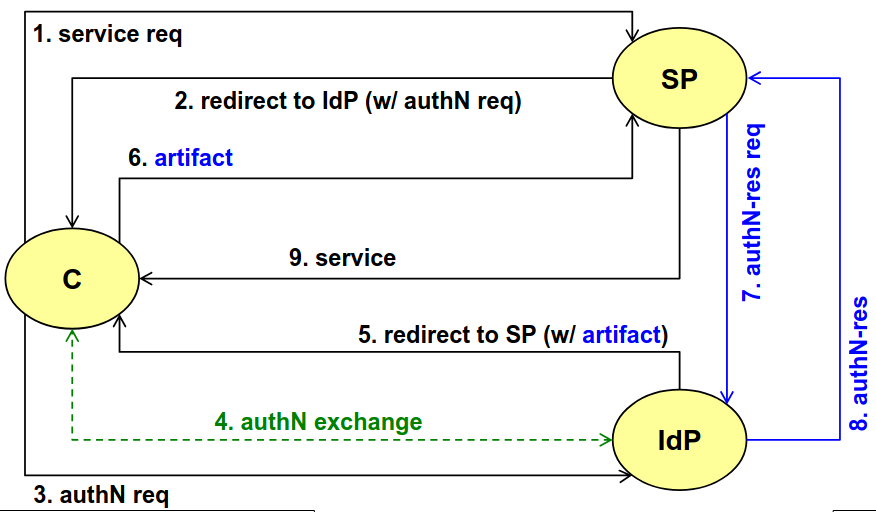
\includegraphics[width=0.5\textwidth]{img/sso pull use case.png}
  \caption{SSO pull use case}
\end{figure}

\subsection{SAML SSO for Google Apps}
This kind of architecture is being used by large providers such as
Goggle to implement SSO for Google Apps.

Google Apps are applications that are hosted by Google, but the
authentication and the authorization are managed by the company that
developed the app. The company asks to Google to run applications on
Google but with the possibility to manage the authentication (so the
company does not want to use Google authentication) in order to keep
control on who is accessing”. This can be performed using SAML.

A company, basically a Google Partner, installs its own applications
on Google (which will be just a service provider). The Partner wants
to maintain control of the authentication and authorization part
(basically the company wants to be an Identity Provider). The exchange
is based on SAML-2.0 with XML signature: this is important because
here there are two difference companies and Google wants to be sure
that any mistake about the authentication cannot be on charge of
Google. This is the typical case in which a signature is needed,
typically a digital signature with X.509 certificate, because in case
of any commercial discussion or legal discussion between Google and
the company, Google wants to have a proof of why they permitted access
to the application.

Basically, there is Google with the Application. All the users that
want to use the application are redirected to the company. Then there
will be the SAML assertion sent to Google which must be digitally
signed, since that is the message that gives access to the application
from Google to the user. If an assertion is accepted without any
signature (or with a symmetric signature), then there is no way to
prove that.

\begin{figure}[H]
  \centering
  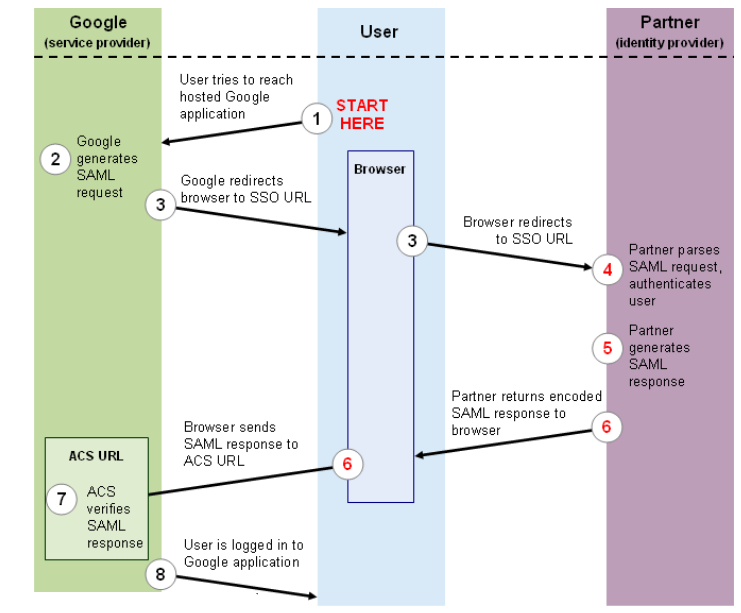
\includegraphics[width=0.7\textwidth]{img/google sso.png}
  \caption{SAML SSO for Google Apps}
\end{figure}

The partner must provide to Google the URL of the single-sign-on
service that can be also named the IDP, or the Authentication Server,
as you prefer, and the X.509 certificate to verify the signature.
Because the answer is signed with a real public key. Step three
contains, in opaque mode, the URL of the Google service requested by
the user. So the company knows not only, I have to authenticate, they
can also perform authorization. Because this user is trying to use
this service, the SML authentication request. And the URL where to
send the response. And step six, in opaque mode, contains still the
URL of the Google service to avoid a reply.
  
\section{Federated Identity}

So far, we have seen \textbf{Delegated Identity}, which operates
within the same security domain. For example, in the case of PoliTo
(where 100 servers delegate authentication to \texttt{idp.polito.it})
or Google’s delegated authentication model, the authentication is
handled by a specific Identity Provider (IdP) for a specific
application. This setup always involves a one-to-one mapping: one
application corresponds to one IdP. While the same IdP can serve
multiple applications, there is still a 1:1 mapping.

On the other hand, \textbf{Federated Identity} enables multiple IdPs
to interact with the same application service. This is a common
scenario, such as when creating an account on a website where users
can either create a new username and password or authenticate using
Google or Facebook credentials. This federation allows authentication
performed by an external service (outside the security domain) to be
automatically recognized. A key advantage is avoiding
\textit{duplicate authentication}, which can be inconvenient for
users.

Federated Identity extends federated authentication by incorporating
\textbf{identity-related attributes}. SAML is frequently used for
building federated identity systems because it supports both
authentication and attribute assertion. Identity involves more than
just authentication; it includes \textit{authentication + attributes}
(e.g., name, surname, student ID, residence, etc.).

SAML is XML-based. While XML is \textit{simple but heavy}, SAML is
typically suited for PC or server-based environments. However, its
complexity makes it challenging to use in lightweight or mobile
contexts.

There is a juxtaposition between \textbf{SAML} and \textbf{OpenID
Connect}. While SAML works well for server environments, it is less
mobile-friendly. OpenID Connect, on the other hand, provides a similar
architecture involving the client, Service Provider (SP), and IdP, but
it uses \textbf{JSON} instead of XML and relies on the \textbf{REST
protocol}. This makes OpenID Connect more suitable for mobile and web
applications.

\begin{boxH}

\textbf{Beware:} \textit{OpenID 1.0} and \textit{OpenID 2.0} are
\textbf{not} the same as OpenID Connect. The latter is based on
\textbf{OAuth 2.0}, an IETF authorization framework. This distinction
is critical, as the terminology surrounding OpenID can sometimes be
confusing.

\end{boxH}

\subsection{OpenID Connect}
OpenID Connect(OIDC) is a delegated authentication system (the
federated aspect rely in the fact that it support many IdPs).

It uses JSON data and REST protocol(which are native in smartphone
environments), and it is not correlated to OpenID-2.0 but this is an
identity layer put on top of Oauth-2.0 (IETF authorization framework).
It should be the reverse: first authentication then authorization, but
not in this case.

The user agent can be a normal browser o can be a mobile app, beware
of the terms because the client is not the user agent, the client is
the relying party (application server) that wishes to use
OpenID-Connect for authentication.

In this schema the user has its mobile phone, and it is named User-
Agent, which is connecting to an application server, which is the
client, because it is the client of OpenID-connect, connecting to a
server that will provide authentication, authorization, and
attributes. That’s why it is named client because it is the client for
OpenID-connect.

The server S is not a single server, but it is a collection of
servers, or as a minimum a collection of endpoints. It means that when
there is a server with a certain network address, there may be several
different ports or even if everything is on port 80 or port 443, when
performing a GET or POST a path is specified, and that is an endpoint.
There may be \texttt{/authenticate}, \texttt{/authorize},
\texttt{/attributes}: these are different entry points in a REST
application.

Notice that the server, which is the OpenID-Provider (OP), which is
conceptually similar to the IdP, has various endpoints:
\begin{itemize}
  \item Authorization endpoint ($\text{AuthZ}_{EP}$: it is called
    authorization, but it performs authentication (confusing).
  \item Token endpoint ($\text{Token}_{EP}$), something that verifies
    if a certain token generated during the protocol is valid or not.
  \item UserInfo endpoint ($\text{UserInfo}_{EP}$), if the user has
    given the consent, then the client can retrieve information about
    the user.
\end{itemize}

\subsubsection{User authentication}
The login workflow is shown in figure \ref{fig:openid-connect} and is
as follows.

We have the user interacting through a \textbf{user agent}, like a
mobile app or a browser. The \textbf{client} here is the relying party
(RP)—for instance, a web application or a service accessed via the
app. The user begins by choosing to log in using an external IdP, such
as Facebook or Google.

The client generates an \textbf{authentication request} to the IdP.
This request is sent to the IdP’s \textbf{authorization endpoint}, even
though the goal is authentication (this dual-purpose endpoint can
cause some confusion). The request includes details like the client
ID, redirect URI, and requested scopes.

Upon receiving the authentication request, the IdP validates it. This
validation ensures that:

\begin{itemize}
  \item The client (RP) is registered with the IdP (a trusted
    relationship exists).
  \item The request is properly signed and formatted, verifying it
    genuinely comes from the registered client.
\end{itemize}

If the request is valid, the IdP generates an \textbf{authentication
page}. Here, the user enters their credentials (e.g., username and
password). The credentials are submitted back to the IdP’s
\texttt{/authenticate} endpoint, where they are verified.

Once authenticated, the IdP often presents the user with an
\textbf{authorization page}. This page asks the user to consent to the
RP accessing specific data (e.g., profile, email). For example, when
using Google or Facebook login, you might see a message like, "This
app will receive your name, email, and profile picture." 

If the user grants consent, the request is finalized at the
\texttt{/authorize} endpoint. The IdP issues an \textbf{authentication
response}, typically as an ID token (a JSON Web Token, or JWT), which
contains the authenticated user’s information. This token is sent back
to the client via the redirect URI specified earlier.

\subsubsection{Login with token}
The login workflow is shown in figure \ref{fig:openid-connect} and is 
as follows.

It's assumed that the user has already authenticated with the IdP and 
has an active session.
After the redirect from the Authorization Endpoint (AuthZEP), a 
\texttt{GET} request is sent to a \texttt{/callback} endpoint, passing 
the received information. The Authorization Endpoint provided a token 
in response. This token is then handed to the client, which can use it 
at the Token Endpoint (TokenEP) for validation. This demonstrates that 
the user consented to transfer their data to the client. 

The Token Endpoint verifies the token, and if valid, it returns 
\textbf{IDT} (Identity Token) and \textbf{ACCT} (Accessory Information). 
The client verifies the IDT, and if accessory information is present, 
the \textbf{UserInfo Endpoint} (UserInfoEP) may optionally be accessed 
to retrieve additional user details. 

Finally, a successful login occurs, and the client is provided with 
the user's identity and any additional information.

%2 subfigure 
\begin{figure}[H]
  \centering
  \begin{subfigure}{.49\textwidth}
    \centering
    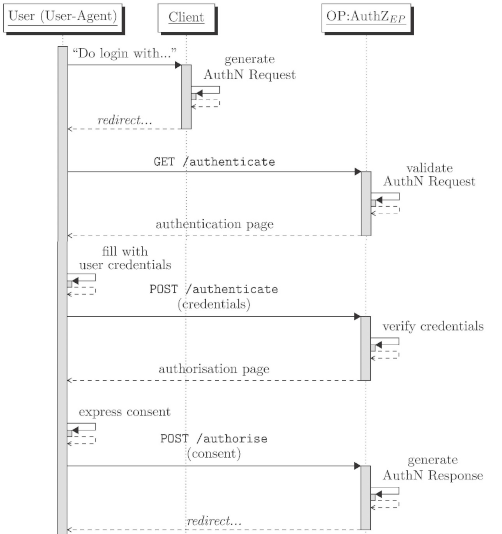
\includegraphics[width=0.9\textwidth]{img/oicd user auth.png}
    \caption{User authentication}
  \end{subfigure}
  \begin{subfigure}{.49\textwidth}
    \centering
    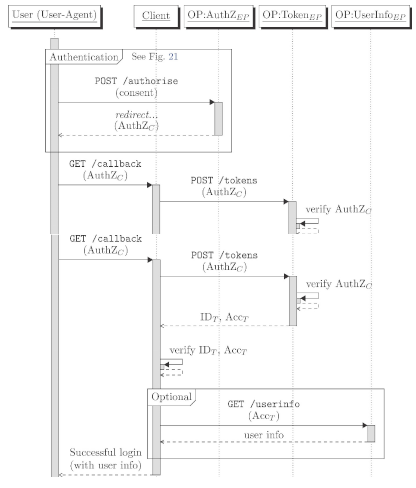
\includegraphics[width=0.9\textwidth]{img/oicd token login.png}
    \caption{Login with token}
  \end{subfigure}
  \caption{OpenID Connect}
  \label{fig:openid-connect}
\end{figure}

\subsubsection{Trust, security and discovery}
All the messages are authenticated with digital signatures, that
requires registration of the public keys among the various actors. All
the messages are protected via secure channel (TLS) but this is not a
real federation, it is just the fact that it is possible to use more
than one. There is a proposed service, WebFinger, to discover the
OpenID Providers but that works only if the provider registered itself
with WebFinger, so it is not much used. But in any case, OpenID
Connect is much used, OIDC providers: Google, Facebook, Salesforce.

\subsubsection{OIDC standard claims}
When additional information about user is requested, it is possible to
ask for:
\begin{itemize}
  \item profile category: subject (ID at the issuer), name (full),
    given\_name, family\_name, middle\_name, nickname,
    preferred\_username, gender, birthdate, zoneinfo, locale, profile
    (URI), picture (URI), website (URI), updated\_at (last update at the
    issuer)
  \item email category: email, email\_verified (Boolean)
  \item phone category: phone\_number, phone\_number\_verified (Boolean)
  \item address category: address
\end{itemize}
When a client is requesting a claim, it may request a single item or a
whole category (e.g., profile category or only family\_name). Apart
from the ones with \_verified=TRUE all the others are self-asserted by
the user and hence unreliable. This is the bad part: the user can be a
fake user. Custom claims can be created, but they have a restricted
audience.

\subsubsection{JWT for claims – example of ID token}
There is: the subject, the issuer (the OpenID connect at PoliTo), the
audience (which client, it can be also www.unito.it because that
server can be a client to accept the user of PoliTo rather than
forcing them to have an account at that website), the nonce, the
authentication time, the authentication context class reference (it is
a way to explain which kind of authentication was performed, of course
some values must be agreed which could be PoliTo, loa stands for level
of assurance and hisec could be high security but there should be a
meaning, a definition behind that), the issued at (at what time the
token was created), the expiration (when it will expire).

\begin{figure}[H]
  \centering
  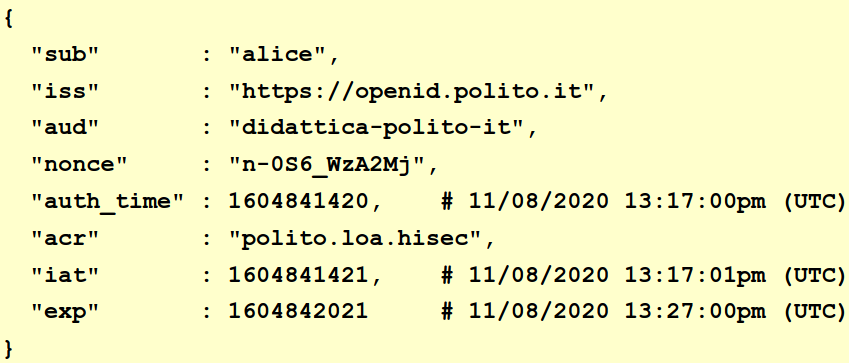
\includegraphics[width=0.5\textwidth]{img/oicd token.png}
  \caption{Example of ID token}

\end{figure}

\section{eIDAS}

\textbf{eIDAS}, stands for \textit{electronic IDentification, Authentication, 
and trust Services for electronic transactions in the internal
market}, and it's based on the EU regulation 910/2014.

The key point is that in each European country there is a different
identity system (in Italy SPID) but in the same way in which the
identity card, the driving license, the passport is valid also on
abroad, the European Union wanted to allow the use of the electronic
identity when accessing services in a different European country. It
took a lot of years (more then 10 years) and it works and it is used
all over Europe.

Initially, the eIDAS electronic identification (eID) infrastructure was 
voluntary. However, starting from September 2018, it became compulsory for 
EU public services. Adoption by the private sector remains optional but is 
strongly encouraged.

The purpose is to boost confidence and trust towards digital world by
adopting the following principles among others:
\begin{itemize}
  \item Mutual acceptance of national e-ID: all the members of EU are
    trusted
  \item Common framework for secure interaction between citizens,
    companies, and public administration
  \item Technological neutrality of requirements Required to not
    restrict to specific solutions (some countries use smartcards,
    others OTP, etc.). All the solutions are mutually recognized, but
    it is not possible to say all the methods are equivalent.
  \item Level of trust in national electronic identity can be defined
    by a certain e-ID quality level
  \item Country-specific supervision organizations to verify the
    Regulation adoption and interact with the European Commission
    (e.g., for data privacy)
\end{itemize}

There were various implementing acts made by Commission Implementing
\begin{itemize}
  \item 2015/296 (24 February 2015): eID procedural arrangement for
    MS(Member state) cooperation
  \item 2015/1501 (8 September 2015):  interoperability framework
  \item 2015/1502 (8 September 2015): technical specifications for
    assurance levels for electronic identification means
  \item 2015/1984 (3 November 2015):  formats and procedures for
    notification
\end{itemize}

\subsection{Pan-European eID}
Notice once again that identity is not just authentication, it is
\textbf{authentication plus attributes}. The very important point is
the fact that with eIDAS there are certified attributes. In OpenID
Connect there are a lot of information, but only phone number and
email can be trusted, since all the others are self-declared by user.
On the contrary, in eIDAS, since the information is provided by the
government it is trusted. 

So, again in eIDAS there will be e-identity with authentication +
certified attributes
\begin{itemize}
  \item Set of certified European attributes
  \item Lexicon (multilanguage attribute names): it is a problem,
    since all the countries in the EU must agree (due to different
    alphabets and characters).
  \item Syntax (possible values)
  \item Semantics e.g., surname in Italy is just one given by the
    father but in Island there are two surnames, since each person
    keeps both surname of father and mother and they can decide to use
    one or the other. So, it is needed to understand the different
    meaning that even simple things may have in different countries.
\end{itemize}

It is possible to use various authentication credentials such as
reusable password, one-time-password, cellphone, software certificate,
smart-card since the system is technology neutral. The point is that
it is used in a transparent way and with legal value (according to the
citizen’s country).

\subsection{Adaptive security and privacy protection}
Everything is accepted but each authentication method it is assigned
various authentication levels and the authentication level is
attributed through the LOA (Level of Assurance) which means how much
the result (on the authentication method) can be trusted. LOA consists
in three different levels: substantial, medium, high. This is not only
related to the cryptographic strength of the authentication technique,
but also on the strength of the identification process, because e.g.,
a country is using a smart-card with a PKC asymmetric
challenge-response which is the strongest authentication, but how does
the smart-card is given to the citizen? If there is no identification
of the citizen, then it is bad. In the end, the LOA tests both things
in order to give a level to the whole procedure.

When accessing a service there may be a mismatch (e.g., a service is
for transferring money so an High LOA is wanted) if the procedure
provides a Medium LOA but the service requires an High LOA, so
authentication may fail.

For privacy protection and localization, the user talks with its own
country and before transferring attributes abroad, it must provide
explicit consent for the required attributes. The attributes are
managed end-to-end, which means that attributes are transferred from
the government of a country directly to the Service Provider in the
other country: eIDAS infrastructure itself does not store any personal
data. There is minimal disclosure, in the sense that on the contrary
to OpenID Connect in which everything can be requested, in this case
it is applied the Need-To-Know principle, e.g., some services are
reserved to people with age major than 18: in this case the birth date
is not requested, since the service is not interested to that
information but the service will ask to the system if the user is
above 18 or not.

\subsection{eIDAS terminology}
The MS is the Member State. It can be:
\begin{itemize}
  \item Sending MS: it is the MS whose eID scheme is used in the
    authentication process, and sending authenticated ID
  \item Receiving MS: it is the MS where the RP requesting an
    authentication (service that citizen is trying to access) is
    established
\end{itemize}
Then there is an eIDAS-Connector, which is a node requesting a
cross-border authentication and the eIDAS-Service which is a node
providing cross-border authentication. Unfortunately, there are two
implementations.

One big country in Europe did not want to agree with the others, so
99\% of countries implements the eIDAS- Proxy-Service (an eIDAS-Service
operated by the Sending MS and providing personal identification data)
schema, while one country is implementing it using
eIDAS-Middleware-Service (an eIDAS-Service running Middleware provided
by the Sending MS, operated by the Receiving MS, and providing
personal identification data) schema.

\subsection{eIDAS infrastructure}
Imagine to be an Italian citizen with SPID identity that needs to
access a SP in Sweden. The SP will ask to the citizen to choose
between the Swedish identifier or eIDAS for authentication. The
citizen will of course choose eIDAS, so it will be redirected to the
Swedish eIDAS Connector (which connects that country to the rest of
the infrastructure). It will ask to select the country of the citizen
and will then redirect to the Italian eIDAS Service which is
implemented as a proxy. At this point the proxy will provide to the
citizen all the information that Sweden requested (name, surname, date
of birth) and will ask for a preliminary consent (otherwise the
process will stop). Then, since in Italy there are different systems
for identity (SPID, but with many providers such as Poste Italiane and
it could be possible to use the electronic identity card) the citizen
must choose which electronic identifier (e-ID) to use. In this way the
citizen will be redirected to that specific provider, which has got
the identity and the attributes (IDP + AP). At this point, the
authentication will be performed according to the system selected and
there will be a final consent to transfer abroad the specified
information (again name=”Antonio”, surname=”Lioy”, etc.).

\begin{figure}[H]
  \centering
  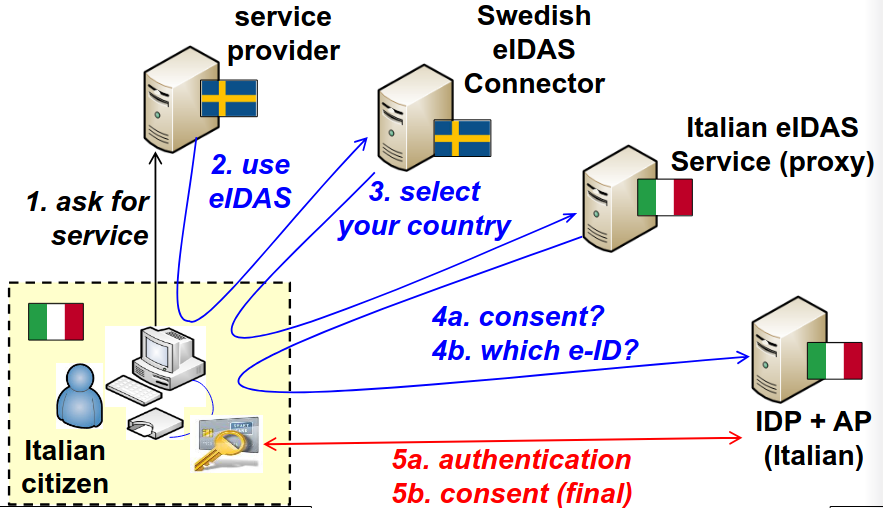
\includegraphics[width=0.5\textwidth]{img/eidas infrastructure.png}
  \caption{eIDAS infrastructure}
\end{figure}
\subsection{eIDAS technical specifications}
Technical specifications are evolving over the time: Version 1.0
(26/01/2016), 1.1 (16/12/2016), Version 1.2 (27/09/2019). They are all
publicly available on the European website. The protocol is based on
STORK1 and then STORK2, that are developed and tested infrastructure
and finally after STARK2 everything was adopted as the official eIDAS
Infrastructure. It is similar, but not compatible, e.g., in the real
implementation it has been added the encryption of authentication
response to guarantee privacy against network sniffing. It covers, but
only for the international part, i.e., MS-to-MS. Looking the previous
picture, eIDAS in the part 3 (Connector exiting from one country and
the proxy accepting request from the other country). Specification is
only for this part (how SPID works in Italy it is decided by Italian
Government, …). eIDAS is end-to-end conceptually, in the sense that
the response will directly transfer to the SP but as a protocol, it is
only for connecting the end-points at the borders of the various
countries. It covers, only for the international part, the:
\begin{itemize}
  \item Interoperability architecture
  \item SAML message format
  \item SAML attribute profiles
  \item Cryptographic requirements
\end{itemize}
\subsubsection{eIDAS Minimum Data-Set}

The eIDAS regulation specifies a minimum data-set that must be supported by any eIDAS node to enable cross-border authentication. This data-set includes attributes for both natural and legal persons.

For \textbf{natural persons}, the data-set includes:
\begin{itemize}
    \item \textbf{Mandatory Attributes:}
    \begin{itemize}
      \item \texttt{PersonIdentifier}, \texttt{FirstName},
        \texttt{FamilyName}, \texttt{DateOfBirth}
    \end{itemize}
    \item \textbf{Optional Attributes:}
    \begin{itemize}
        \item \texttt{BirthName}, \texttt{PlaceOfBirth},
          \texttt{CurrentAddress}, \texttt{Gender}
    \end{itemize}
\end{itemize}

For \textbf{legal persons}, the data-set includes:
\begin{itemize}
    \item \textbf{Mandatory Attributes:}
    \begin{itemize}
        \item \texttt{LegalName}, \texttt{LegalPersonIdentifier}
    \end{itemize}
    \item \textbf{Optional Attributes:}
    \begin{itemize}
        \item \texttt{LegalAddress} , \texttt{VATRegistration} ,
          \texttt{TaxReference} , \texttt{BusinessCodes} ,
          \texttt{LEI} (Legal Entity Identifier) , \texttt{EORI}
          (Economic Operators Registration and Identification) ,
          \texttt{SEED} (System for Exchange of Excise Data) ,
          \texttt{SIC} (Standard Industrial Classification)
    \end{itemize}
\end{itemize}

\subsubsection{Security Requirements}

\begin{itemize}
    \item \textbf{SAML request} (no personal data) \textbf{MUST} be
      signed with a digital signature, but no encryption is required.
    \item The request may be transmitted via:
    \begin{itemize}
        \item \textbf{HTTP Redirect}: For example, a 302 GET with the
          request in a parameter. This is preferred if the size of the
          request does not exceed the maximum URI length (256
          characters).
        \item \textbf{HTTP POST}: For example, a form with POST and
          the request in a hidden field. This is preferred if the
          request is much larger.
        \item Note: The size of the request can change based on the
          data requested. For instance, authentication requests with
          attributes will make the request larger.
    \end{itemize}
    \item \textbf{SAML response} (containing personal data)
      \textbf{MUST} be signed with a digital signature and must
      include an \texttt{EncryptedAssertion} with:
    \begin{itemize}
        \item One \texttt{AuthenticationStatement}
        \item One \texttt{AttributeStatement}
    \end{itemize}
    The response itself is not encrypted, but portions of it may be
    encrypted as allowed in SAML.
    \item The response is transmitted via \textbf{POST binding} to the
      ACS (\textit{Assertion Consumer Service}) of the connector.
    \item The connector metadata must contain:
    \begin{itemize}
        \item The \textbf{encryption certificate} and \textbf{ACS URI}.
        \item For example, when Italy sends back encrypted data, it
          needs to know the public certificate and the ACS URI to
          perform a redirect after authentication. These details are
          included in the metadata.
    \end{itemize}
\end{itemize}

\textbf{All communication channels must use TLS version $\geq$ 1.2,
with qualified web certificates.} The supported TLS ciphersuites are:
\begin{itemize}
    \item ECDHE+ECDSA or ECDHE+RSA or DHE+DSA (accepted for backward
      compatibility)
    \item AES\_128\_CBC/GCM with SHA256 for encryption
    \item AES\_256\_CBC/GCM with SHA384 for encryption
    \item SHA1 MAY be accepted but only due to restrictions of the
      client browser
\end{itemize}

Other Requirements for TLS:

\begin{itemize}
    \item For \textbf{ECDH keys}, the minimum key size is 256 bits,
      while for \textbf{DH keys} the minimum is 2048 bits.
    \item The \textbf{TLS compression} \textbf{SHOULD NOT} be used.
    \item \textbf{TLS heartbeat} and \textbf{Session Renegotiation}
      \textbf{MUST NOT} be used.
    \item If a \textbf{CBC-based cipher suite} is used, first encrypt
      and then authenticate the data (e.g., use the Enc-then-MAC
      extension).
    \item \textbf{DON'T} use a truncated HMAC (e.g., unsupported that
      extension).
\end{itemize}

Requirements for SAML:

\begin{itemize}
    \item \textbf{Data encryption} only via \texttt{AES-128/256-GCM},
      but \texttt{AES-192-GCM} may also be used.
    \item \textbf{Key encryption} with \texttt{RSA-OAEP-MGF1P} or
      \texttt{RSA-OAEP} (3072 bits minimum key length).
    \item \textbf{Key agreement} via \texttt{ECDH-ES}:
    \begin{itemize}
        \item \texttt{ES} is \textit{Ephemeral-Static mode} (i.e., the
          recipient has static DH parameters while the sender creates
          ephemeral ones). The destination publishes in the metadata
          what its own DH parameters are, while the sender will create
          the ephemerals.
    \end{itemize}
    \item \textbf{Key wrapping} via \texttt{KW-AES-128/256}.
    \item \textbf{Digital Signature} via \texttt{RSAPSS} (3072 bits
      minimum key length) or \texttt{ECDSA} (256 bits minimum key
      length) with \texttt{SHA-256/384/512}.
    \item The trusted EC are: \texttt{BrainPoolP256r1,
      BrainpoolP384r1, BrainpoolP521r1, NIST Curve P-256, NIST Curve
    P-384, NIST Curve P-521}.
\end{itemize}

\subsection{eIDAS 2.0}

eIDAS 2.0 introduces a new schema based on the \textbf{EUDI} (EU
Digital Identity) wallet. It implements the concept of \textbf{SSI}
(Self-Sovereign Identity). The EUDI wallet will provide identification
and authentication, as well as the verifiability of the validity of
the evidence by third parties throughout Europe. It ensures secure
storage and presentation of verified identities and their data, and
enables the generation of qualified electronic signatures.


\section{SPID}
SPID is the Italian Public System for Digital Identity. It's
architecture is based on three main components:
\begin{itemize}
  \item \textbf{Identity Provider (IdP)}: the entity that provides
    digital identity to the user. It is responsible for the
    authentication process and the enrollment of the user.
    It also returns the user identity plus some basic attributes(not
    all of them).
  \item \textbf{Service Provider (SP)}: the entity that performs
    access control based on the identity and attributes. 
  \item \textbf{Attribute Authority (AA)}: the entity that provides
    the user's attributes based on the identity. This is necessary
    there are some attributes that are not controlled by the
    government, for instance the enrollment to the \textit{Ordine
    degli Ingegneri}.
\end{itemize}

\subsection{Protocols and data}
SPID uses SAML version 2 with the web browser SSO profile for data
exchange. The caveat is that each entity prodives its own metadata,
containing:
\begin{itemize}
  \item its X.509 signature certificate, which may be self-signed!
    This is possible because the metadata is public and can be 
    accessed from a goverment controlled website.
  \item its protocol endpoints
  \item various other data (e.g. supported attributes)
\end{itemize}

The metadata are signed by the Agency for Italian Digitalization in
detached form. This means that they will be the target of electronic
signatures. The official metadata registry containing all the service
providers and identity providers can be found at 
\url{https://registry.spid.gov.it/metadata}. The specification in case
of spid are a little bit behind the eIDAS, because the basic signature
algorithm is RSA-2048 with sha-256, while eIDAS requires RSA-3072 
with sha-384.

In case of an HTTP redirect, the SAML request is passed in the query
string of a GET. But this has a limit of 256B for the basic URI, but
typically length of 2kB up to 8kB are supported. Since POST requests
are not to be used, the SAML request is compressed with DEFLATE 
algorithm and not signed with SMLDSIG, but the SigAlg parameter is
used to specify the signature algorithm, in a Base64 url encoded form
of the whole query string. When using HTTP POST, then we permit normal
SAML with normal XML signature.

There are many basic attributes, and each SP may require a specific
attribute set, which groups them. A common example of an attribute set
could be (name, familyName,  fiscalNumber, email).

There are also different authentication levels:
\begin{itemize}
  \item SPID Level 1: the user is authenticated with a password
  \item SPID Level 2: the user is authenticated with a password and OTP
    or password and an app
  \item SPID Level 3: this level requires 2FA with asymmetric authN
    via a secure device, for example a password with an app for remote
    digital signature and a Layer 3 pin
\end{itemize}

\subsection{SPID evolution}
The Attribute Authority is not yet implemented, but it's not for a
technical issue, but an organizational one: the government has not
decided who is authorized to create some attributes.

There's also a requesto make SPID available not only with SAML, but
also with OIDC, to make it more compatible with the rest of the world.
This is compulsory for the IDPs since May 1, 2022. For the service
provider, it is optional to support that.


\section{Q\&A}
\subsection*{Question 1}
what role does the Authentication Server (AS) play?
\begin{itemize}
  \incorrect provides authorization decisions for the RP
  \correct performs authentication on behalf of the Relying Party (RP)
  \incorrect verifies the identity of the RP
  \incorrect issues a session timeout for the RP
\end{itemize}

\subsection*{Question 2}
\begin{itemize}
  \incorrect relaying party is A. the entity that directly authenticates the user 
  \incorrect  the server that stores user credentials
  \correct  the entity that trusts another server to handle authentication
  \incorrect  the client application used by the user
\end{itemize}

\subsection*{Question 3}
the Authentication Server (AS) interacts with the client using
specific protocols to perform authentication. What amongst the
following can be used for the authentication process
\begin{itemize}
  \incorrect HTTP 
  \correct OAuth 
  \incorrect FTP
  \incorrect SMTP 
  \correct SAML 
  \incorrect SOAP
\end{itemize}

\subsection*{Question 4}
how does the Authentication Server (AS) typically
communicate the authentication result to the Relying Party (RP)?
\begin{itemize}
  \incorrect  by issuing an authorization code 
  \incorrect  by sending a cookie
  \correct  by providing a ticket or assertion 
  \incorrect  by creating a session ID
\end{itemize}

\subsection*{Question 5}
Which of the following scenarios best represents a delegated authentication setup in a Single Sign-On (SSO) environment
\begin{itemize}
  \incorrect  the user logs in separately to each application with the same credentials
  \correct the user logs in once, and a central AS authenticates them for multiple RPs
  \incorrect each application has its own AS that verifies the user separately
  \incorrect the user must verify their identity with each RP individually
\end{itemize}

\subsection*{Question 6}
Which format is commonly used to provide assertions in delegated authentication systems like SAML?
\begin{itemize}
  \incorrect  JSON Web Tokens (JWT)
  \incorrect  Hypertext Markup Language (HTML) 
  \correct  Extensible Markup Language (XML) 
  \incorrect  Simple Mail Transfer Protocol (SMTP)
\end{itemize}

\subsection*{Question 7}
Which of the following is a key benefit of using delegated authentication for a Relying Party (RP)?
\begin{itemize}
  \incorrect  reduced dependency on external servers 
  \correct  enhanced data privacy for user credentials 
  \incorrect  increased complexity in user management 
  \incorrect  independent authentication for each RP
\end{itemize}

\subsection*{Question 8}
what does a SAML assertion represent?
\begin{itemize}
  \correct  declaration of a fact about a subject, like user information
  \incorrect  a statement about of how often a user logs in
  \incorrect  a protocol for secure email communication
  \incorrect  a form of encryption used for securing passwords
  \incorrect  a method of encoding data in XML format
  \correct  declaration made by an issuer about a different subject
\end{itemize}

\subsection*{Question 9}
Which of the following is not a standard type of SAML assertion?
\begin{itemize}
  \incorrect  authentication assertion
  \correct  Service type assertion
  \incorrect  authorization decision assertion 
  \correct  public key certificate assertion 
  \incorrect  attribute assertion
  \correct  token assertion
\end{itemize}

\subsection*{Question 10}
When an Identity Provider (IdP) issues a SAML assertion, who is
typically the recipient that relies on this assertion?
\begin{itemize}
  \incorrect user's web browser
  \correct Relying Party (RP)
  \correct Service Provider (SP)
  \incorrect DNS server
  \incorrect certificate authority 
  \incorrect password manager
\end{itemize}

\subsection*{Question 11}
Why does SAML use XML as the standard format for its assertions?
\begin{itemize}
  \correct  XML provides a flexible, readable format for exchanging
  information across systems
  \incorrect  XML is universally adored by data specialists 
  \incorrect  XML is the default because JSON was too complicated
  \correct  XML allows for custom-defined tags, which means SAML can
  extend its structure to include additional fields or attributes as
  needed without breaking compatibility with existing systems
  \incorrect  XML prevents other formats from being easily implemented 
  \incorrect  XML encodes information only in binary for extra security
  \correct  XML allows SAML to be platform-independent and easily
  parsed by different systems 
\end{itemize}

\subsection*{Question 12}
In policy-based access control (PBAC), what is the primary function of
the Policy Enforcement Point (PEP)?
\begin{itemize}
  \correct enforces access to a resource based on the policy decision 
  \incorrect collects user attributes for policy decision-making
  \incorrect decides whether a policy is applicable to a specific
  access request
  \incorrect acts as a backup in case the Policy Decision Point (PDP)
  fails
  \incorrect protects resources by ensuring they're only accessed when
  policies align with user attributes
\end{itemize}

\subsection*{Question 13}
Which of the following best describes the role of the Policy Decision
Point (PDP) in PBAC?
\begin{itemize}
  \incorrect enforces access controls based on predefined policies
  \incorrect collects and provides the necessary policies for the reguested access
  \correct evaluates all information (policy, subject, resource, and access type) to determine if access should be granted
  \incorrect monitors user behavior and access patterns for anomaly detection
  \incorrect checks user permissions, but only on days when its not overloaded
  \incorrect none of the above
\end{itemize}

\subsection*{Question 14}
What is the primary purpose of a SAML binding?
\begin{itemize}
  \correct to specify the underlying protocol used to transport SAML
  reguests and responses
  \incorrect to define how SAML assertions are signed for security purposes
  \incorrect to describe the format of SAML messages exchanged between
  systems
  \incorrect to establish a fallback protocol for non-compliant systems
  \incorrect to ensure SAML messages are transported using the fastest
  possible route
\end{itemize}

\subsection*{Question 15}
Which of the following is not a valid SAML binding?
\begin{itemize}
  \incorrect  SAML SOAP binding
  \incorrect Reverse SOAP (PAOS) binding
  \incorrect  HTTP POST binding
  \correct FTP-over-SAML binding
  \incorrect  HTTP redirect binding
  \correct  SAML-over-TLS binding
\end{itemize}

\subsection*{Question 16}
In the SAML SOAP binding, what role does SOAP play?
\begin{itemize}
  \incorrect  It formats the SAML reguest/response messages in XML for
  transmission
  \incorrect  It determines the security of the SAML assertion being
  transported
  \correct  It wraps SAML messages inside a SOAP envelope over HTTP
  \incorrect  It acts as an intermediary to deliver SAML assertions
  across different servers
  \incorrect  It ensures messages are "clean and shiny" before they'Tre
  sent
\end{itemize}
